% !TEX root = ../main.tex
\chapter{Matematiske verktøy vi trenger}
\intro{I fysikk bruker vi matematikken som et presist språk for å beskrive verden rundt oss. Her ser vi på de viktigste matematiske verktøyene du trenger i dette kurset. Det betyr ikke at vi går nøye gjennom alt, men kapitlet gir en oversikt over de grunnleggende konseptene og reglene du bør være komfortabel med.}
\tanke{}{%
Hvorfor kan naturen beskrives med matematikk?}

\begin{mymerk*}{Python og programmering}
I dette kompendiet bruker vi Python for å illustrere beregninger og lage figurer. Om du aldri har programmert før, anbefaler vi å lese Appendiks~\ref{app:python} før du går videre. Der finner du en kort innføring i alt du trenger for å komme i gang.
\end{mymerk*}

\section{Algebra}

Algebra handler om å uttrykke sammenhenger mellom størrelser ved hjelp av variabler og symboler. I stedet for å skrive at «fart er strekning delt på tid» kan vi skrive den mer presise formelen
\[
v = \frac{s}{t}.
\]
Her er $v$, $s$ og $t$ \emph{variabler} — symboler som kan settes lik ulike tallverdier.

\subsection*{Noen grunnleggende regler}
\begin{itemize}
    \item \textbf{Regnerekkefølge:} Parentes $\to$ Potens $\to$ Gang/del $\to$ Pluss/minus.
    \item \textbf{Likningslæren:} Det man gjør på én side av et likhetstegn, må man gjøre på begge.
    \item \textbf{Potenser:} $x^a \cdot x^b = x^{a+b}$, \quad $\dfrac{x^a}{x^b} = x^{a-b}$, \quad $(x^a)^b = x^{ab}$.
    \item \textbf{Kvadratrot:} $\sqrt{x} = x^{1/2}$.
\end{itemize}
Noe av det vi kommer til å gjøre mest i fysikken er å sette opp likninger og løse for en variabel; en såkalt "ukjent". La oss ta Newtons 2. lov som eksempel, og se hvordan vi kan løse for akselerasjonen $a$ når vi kjenner kraften $F$ og massen $m$.
\exm{Løse for ukjent}{Newtons 2. lov sier $F = m \cdot a$. En bil med masse $m = 1\,200\ \textrm{kg}$ utsettes for en kraft $F = 4\,800\ \textrm{N}$. Finn akselerasjonen $a$.

\paragraph{Løsning:} Del begge sider på $m$:
\[
a = \frac{F}{m} = \frac{4\,800\ \textrm{N}}{1\,200\ \textrm{kg}} = 4.0\ \textrm{m/s}^2.
\]
}

I eksemplet nedenfor beregner vi den kinetiske energien $E_k = \frac{1}{2}mv^2$ med Python. Merk at koden er veldig lik ordinær algebra — vi definerer variablene og regner ut uttrykket:

\exm{Kinetisk energi}{%
Beregn den kinetiske energien til en gjenstand med masse $m = 2.0\ \textrm{kg}$ som beveger seg med fart $v = 5.0\ \textrm{m/s}$.
\paragraph{Løsning:} Vi bruker formelen for kinetisk energi: $E_k = \frac{1}{2}mv^2$, og bestemmer oss for å bruke Python som kalkulator. Vi definerer variablene $m$ og $v$, og regner ut $E_k$:
}
\begin{pythonkode}
# Kinetisk energi: E_k = 0.5 * m * v**2
m = 2.0    # masse i kg
v = 5.0    # fart i m/s

E_k = 0.5 * m * v**2

print(f"Kinetisk energi: {E_k} J")
\end{pythonkode}
\begin{pythonoutput}
Kinetisk energi: 25.0 J
\end{pythonoutput}

\begin{mymerk*}{Kjøre koden selv}
Alle kodeeksempler finnes som Jupyter Notebook-filer i mappen \texttt{Python eksempler}. Se Appendiks~\ref{app:python} for hvordan du åpner og kjører dem.
\end{mymerk*}

\oppgave{Algebra og Python}{%
\begin{enumerate}[a)]
    \item Beregn $\dfrac{15 + 3^2}{6 - 2}$ for hånd, og sjekk svaret med Python.
    \item Bruk Python til å beregne potensiell energi $E_p = m \cdot g \cdot h$ for $m = 5.0\ \textrm{kg}$, $g = 9.81\ \textrm{m/s}^2$ og $h = 10.0\ \textrm{m}$.
\end{enumerate}
}

\begin{myoppsum*}{Algebraregler}
    \begin{itemize}
        \item Det du gjør på ett ledd må du gjøre på alle ledd i enlikning.
        \item Husk at du alltid kan multiplisere med 1.
    \end{itemize}
\end{myoppsum*}

\section{Funksjoner og plotting}

En \emph{funksjon} er en regel som til enhver innverdi $x$ knytter én bestemt utverdi $f(x)$. I fysikk er funksjoner et sentralt verktøy — for eksempel er posisjonen til et objekt i bevegelse en funksjon av tid.

\subsection*{Lineær funksjon}
Den enkleste funksjonen er den lineære:
\[
f(x) = ax + b,
\]
der $a$ er \emph{stigningstallet} (hvor bratt grafen er) og $b$ er \emph{konstantleddet} (der grafen skjærer $y$-aksen).

\subsection*{Kvadratisk funksjon}
En kvadratisk funksjon har formen
\[
f(x) = ax^2 + bx + c.
\]
Grafen er en parabel. Posisjonen til et legeme med konstant akselerasjon er for eksempel en kvadratisk funksjon av tid: $x(t) = x_0 + v_0 t + \frac{1}{2}at^2$.

\subsection*{Plotting med Python}
En av de nyttigste tingene vi kan gjøre med Python, er å tegne grafer. Eksemplet under plotter posisjon og fart som funksjon av tid for et legeme med konstant akselerasjon:

\begin{pythonkode}
import numpy as np
import matplotlib.pyplot as plt

# Parametre
a  = 2.0    # akselerasjon [m/s^2]
v0 = 0.0    # startfart [m/s]
x0 = 0.0    # startposisjon [m]

# Tid fra 0 til 5 sekunder (200 punkter)
t = np.linspace(0, 5, 200)

# Bevegelsesligninger
x = x0 + v0*t + 0.5*a*t**2   # posisjon
v = v0 + a*t                  # fart

# To grafer side om side
fig, (ax1, ax2) = plt.subplots(1, 2, figsize=(10, 4))

ax1.plot(t, x, color='royalblue', linewidth=2)
ax1.set_xlabel('Tid [s]')
ax1.set_ylabel('Posisjon [m]')
ax1.set_title('Posisjon vs. tid')
ax1.grid(True, alpha=0.3)

ax2.plot(t, v, color='tomato', linewidth=2)
ax2.set_xlabel('Tid [s]')
ax2.set_ylabel('Fart [m/s]')
ax2.set_title('Fart vs. tid')
ax2.grid(True, alpha=0.3)

plt.tight_layout()
plt.show()
\end{pythonkode}
\begin{figure}[H]
\centering
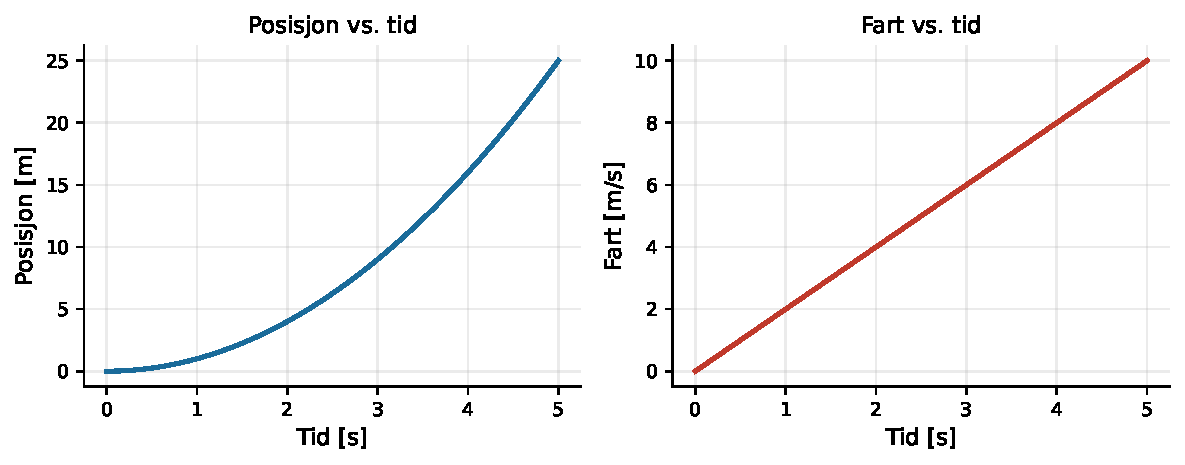
\includegraphics[width=0.95\linewidth]{Images/Kapittel1:introduksjon/python_plot_02_bevegelse.pdf}
\caption{Posisjon og fart som funksjon av tid for konstant akselerasjon $a=2.0\ \textrm{m/s}^2$, $v_0 = 0$.}
\end{figure}

\oppgave{Funksjoner og plotting}{%
\begin{enumerate}[a)]
    \item Bruk Python til å plotte funksjonen $f(x) = 2x^2 - 3x + 1$ for $x \in [-2,\, 4]$.
    \item Modifiser koden over slik at startfarten er $v_0 = 3.0\ \textrm{m/s}$. Hva forandrer seg i grafene?
\end{enumerate}
}

\section{Trigonometri}

Trigonometri handler om sammenhengene mellom vinkler og sidelengder i en rettvinklet trekant. I fysikk bruker vi dette \textit{hele tiden} — særlig for å dekomponere vektorer i komponenter, og for å gå fra størrelse og vinkel tilbake til komponentform.

\subsection*{Den rettvinklede trekanten}

I en rettvinklet trekant navngir vi sidene i forhold til en valgt vinkel $\theta$:
\begin{itemize}
    \item \textbf{Hypotenus} ($h$) — den lengste siden, alltid overfor den rette vinkelen
    \item \textbf{Hosliggende katet} — siden som grenser til $\theta$
    \item \textbf{Motstående katet} — siden overfor $\theta$
\end{itemize}

\begin{center}
\begin{tikzpicture}[scale=1.25, baseline=(current bounding box.center)]
  \coordinate (O) at (0,0);
  \coordinate (A) at (3.2,0);
  \coordinate (B) at (3.2,2);
  \fill[headCol!9] (O) -- (A) -- (B) -- cycle;
  \draw[thick] (O) -- (A) node[midway, below=6pt] {\small hosliggende};
  \draw[thick] (A) -- (B) node[midway, right=5pt] {\small motstående};
  \draw[thick] (O) -- (B) node[midway, above left=2pt] {\small hypotenus $h$};
  \draw (A) ++(-0.22,0) -- ++(0,0.22) -- ++(0.22,0);
  \draw[headCol, thick] (0.55,0) arc (0:32:0.55);
  \node at (0.84,0.14) {$\theta$};
\end{tikzpicture}
\hspace{2.5cm}
\begin{tikzpicture}[scale=1.6, baseline=(current bounding box.center)]
  \draw[->] (-1.2,0) -- (1.3,0) node[right, font=\small] {$x$};
  \draw[->] (0,-1.2) -- (0,1.3) node[above, font=\small] {$y$};
  \draw[thick] (0,0) circle (1);
  \fill[headCol] (0.707,0.707) circle (1.8pt);
  \draw[thick, headCol] (0,0) -- (0.707,0.707)
        node[midway, above left=1pt, font=\small] {$1$};
  \draw[dashed, gray!60] (0.707,0) -- (0.707,0.707);
  \draw[dashed, gray!60] (0,0.707) -- (0.707,0.707);
  \draw[very thick, thmscol] (0,0) -- (0.707,0)
        node[midway, below=4pt, font=\small] {$\cos\theta$};
  \draw[very thick, defscol!80!black] (0,0) -- (0,0.707)
        node[midway, left=4pt, font=\small] {$\sin\theta$};
  \draw[->] (0.28,0) arc (0:45:0.28);
  \node[font=\small] at (0.45,0.13) {$\theta$};
  \node[font=\small, above right=1pt] at (0.707,0.707) {$P$};
\end{tikzpicture}
\end{center}
\begin{center}
\small\textit{Venstre: rettvinklet trekant med vinkel $\theta$. \quad Høyre: enhetssirkelen ($r=1$), der $P=(\cos\theta,\,\sin\theta)$.}
\end{center}

\defn{Sinus, cosinus og tangens}{For en vinkel $\theta$ i en rettvinklet trekant med hypotenus $h$:
\begin{align*}
    \cos\theta = \frac{\text{hosliggende}}{h}, \qquad
    \sin\theta = \frac{\text{motstående}}{h}, \qquad
    \tan\theta = \frac{\sin\theta}{\cos\theta} = \frac{\text{motstående}}{\text{hosliggende}}
\end{align*}
\textit{Huskeregel:} \textbf{Soh-Cah-Toa} — \textbf{S}in = Opposite/Hypotenuse, \textbf{C}os = Adjacent/Hypotenuse, \textbf{T}an = Opposite/Adjacent.
}

Dersom vi kjenner $h$ og $\theta$, gir dette oss katetene direkte:
\[
\text{hosliggende} = h\cos\theta, \qquad \text{motstående} = h\sin\theta.
\]

\subsection*{Viktige verdier}

\begin{table}[H]
\centering
\renewcommand{\arraystretch}{1.55}
\begin{tabular}{|c|c|c|c|}
\hline
\rowcolor{blue!20!black!10}
$\theta$ & $\sin\theta$ & $\cos\theta$ & $\tan\theta$ \\
\hline
$0^\circ$  & $0$ & $1$ & $0$ \\
\hline
$30^\circ$ & $\dfrac{1}{2}$ & $\dfrac{\sqrt{3}}{2}$ & $\dfrac{1}{\sqrt{3}}$ \\
\hline
$45^\circ$ & $\dfrac{\sqrt{2}}{2}$ & $\dfrac{\sqrt{2}}{2}$ & $1$ \\
\hline
$60^\circ$ & $\dfrac{\sqrt{3}}{2}$ & $\dfrac{1}{2}$ & $\sqrt{3}$ \\
\hline
$90^\circ$ & $1$ & $0$ & — \\
\hline
\end{tabular}
\caption{Viktige trigonometriske verdier.}
\label{tab:trig}
\end{table}

\begin{myoppsum*}{Pytagoreisk identitet}
For alle vinkler $\theta$ gjelder:
\[
\sin^2\theta + \cos^2\theta = 1
\]
Dette følger direkte fra Pytagoras' setning brukt på enhetssirkelen.
\end{myoppsum*}

\exm{Trigonometri: stige mot vegg}{En stige av lengde $h = 5.0\ \textrm{m}$ lener seg mot en vegg i vinkel $\theta = 37^\circ$ med gulvet. Finn den horisontale og vertikale komponenten til stigen.

\paragraph{Løsning:}
\begin{align*}
x &= h\cos\theta = 5.0\cdot\cos 37^\circ \approx 5.0\cdot 0.799 \approx \doubleunderline{4.0\ \textrm{m}} \\
y &= h\sin\theta = 5.0\cdot\sin 37^\circ \approx 5.0\cdot 0.602 \approx \doubleunderline{3.0\ \textrm{m}}
\end{align*}
Dette er nøyaktig et $(3,4,5)$-trekant skalert med $1\ \textrm{m}$.
}

\oppgave{Trigonometri}{%
\begin{enumerate}[a)]
    \item Les av $\sin 30^\circ$, $\cos 45^\circ$ og $\tan 60^\circ$ fra Tabell~\ref{tab:trig}.
    \item En kraft $F = 20\ \textrm{N}$ virker i vinkel $\theta = 53^\circ$ over horisonten. Finn de horisontale og vertikale komponentene $F_x = F\cos\theta$ og $F_y = F\sin\theta$.
    \item Vis at $\sin^2 30^\circ + \cos^2 30^\circ = 1$.
\end{enumerate}
}

\section{Vektorer CHECK: Må rydes opp angående koord syst og enhetsvektorer.}
I motsetning til skalarer, som er helt vanlige éndimensjonale tall, er vektorer tall i flere dimensjoner. Vektorer kan ha alt fra to til uendelig mange dimensjoner. I dette kurset skal vi kun arbeide med vektorer i to dimensjoner. Normalt dekomponerer vi vektorer, slik at vi tar for oss en retning om gangen, som gjør det hele mer håndterbart. For å få forståelse for dette skal vi se nærmere på vektorer i $xy$-planet.

\defn{vektor}{En vektor er et objekt med både størrelse og retning.}

\oppgave{Skalarer og vektorer}{%
Er følgende fysiske størrelser skalarer eller vektorer? Begrunn svaret.
\begin{enumerate}[a)]
    \item Temperatur
    \item Kraft
    \item Fart (størrelsen av hastigheten)
    \item Hastighet
    \item Masse
\end{enumerate}
}

\subsection{Enhetsvektorer}

For å arbeide systematisk med vektorer er det nyttig å innføre et sett med faste referansevektorer. Disse kalles \emph{enhetsvektorer} eller \emph{basisvektorer} og definerer retningene i koordinatsystemet. Det som er spesielt med enhetsvektorene, er at alle andre vektorer kan uttrykkes som en lineær kombinasjon av disse.

\defn{Enhetsvektor}{En enhetsvektor er en vektor med lengde 1 som angir en bestemt retning i rommet.}

I $xy$-planet finnes det to enhetsvektorer:
\begin{align}
\hat{\mathbf{x}} = [1,0], \qquad \hat{\mathbf{y}} = [0,1]
\end{align}

Her peker $\hat{\mathbf{x}}$ i positiv $x$-retning, mens $\hat{\mathbf{y}}$ peker i positiv $y$-retning. Sammen danner disse enhetsvektorene grunnlaget for koordinatsystemet.
Merk at $\hat{\mathbf{x}}$ og $\hat{\mathbf{y}}$ er ortogonale, det vil si at de står vinkelrett på hverandre, og at de begge har lengde 1.
\begin{mymerk*}{Alternativ notasjon for enhetsvektorer}
I mange lærebøker brukes symbolene $i$, $j$, $k$ for de samme enhetsvektorene, og noen steder skrives disse med hat som $\hat{i}$, $\hat{j}$, $\hat{k}$. I dette kompendiet bruker vi $\hat{\mathbf{x}}$, $\hat{\mathbf{y}}$ (og $\hat{z}$ i tre dimensjoner), da denne notasjonen gjør det umiddelbart tydelig hvilken retning enhetsvektoren peker i.
\end{mymerk*}

\paragraph{Vektorer skrevet med enhetsvektorer}

Enhver vektor i $xy$-planet kan skrives som en kombinasjon av enhetsvektorene. Hvis vi har en vektor
\begin{align}
\vec{v} = [v_x, v_y],
\end{align}
kan den skrives som
\begin{align}
\vec{v} = v_x \hat{\mathbf{x}} + v_y \hat{\mathbf{y}}.
\end{align}

Denne skrivemåten gjør det tydelig hvordan vektoren er bygget opp av bidrag i hver retning. Tallene $v_x$ og $v_y$ kalles vektorens komponenter.

\paragraph{Hvorfor enhetsvektorer er nyttige}

Enhetsvektorer er spesielt nyttige i fysikk fordi mange lover gjelder uavhengig i hver retning. Ved å dekomponere vektorer i komponenter kan vi derfor analysere et problem én retning om gangen.

For eksempel kan en kraftvektor skrives som:
\begin{align}
\vec{F} = F_x \hat{\mathbf{x}} + F_y \hat{\mathbf{y}}
\end{align}
der $F_x$ og $F_y$ er kraftens komponenter i henholdsvis $x$- og $y$-retning.

Dette gjør det mulig å bruke Newtons lover separat i hver retning, noe som ofte forenkler beregningene betydelig.

\oppgave{Enhetsvektorer}{%
\begin{enumerate}[a)]
    \item Skriv vektoren $\vec{A} = [4,\,-3]$ som en lineær kombinasjon av enhetsvektorene $\hat{\mathbf{x}}$ og $\hat{\mathbf{y}}$.
    \item Regn ut summen $\vec{u} + \vec{v}$ der $\vec{u} = 3\hat{\mathbf{x}} - 2\hat{\mathbf{y}}$ og $\vec{v} = -\hat{\mathbf{x}} + 5\hat{\mathbf{y}}$. Skriv svaret på komponentform.
\end{enumerate}
}

\section{Koordinatsystem}

Et koordinatsystem er et verktøy vi bruker for å beskrive plassering og bevegelse på en presis og entydig måte. Ved å knytte tall til posisjoner kan vi bruke matematikk til å analysere fysiske situasjoner, som for eksempel bevegelse langs en vei, krefter på et legeme eller posisjonen til et objekt i rommet.\\

\defn{Koordinatsystem}{Et koordinatsystem er et matematisk verktøy som gjør det mulig å beskrive fysiske posisjoner og bevegelser ved hjelp av tall.}


I et todimensjonalt koordinatsystem, som $xy$-planet, beskrives en posisjon ved hjelp av et ordnet par $(x,y)$. Her angir:
\begin{itemize}
    \item $x$ posisjonen i horisontal retning
    \item $y$ posisjonen i vertikal retning
\end{itemize}

Punktet $(0,0)$ kalles origo, og fungerer som referansepunkt for alle andre posisjoner i koordinatsystemet.

\oppgave{Koordinatsystem}{%
\begin{enumerate}[a)]
    \item Tegn punktene $A = (2,\,3)$, $B = (-1,\,4)$ og $C = (0,\,-2)$ i et koordinatsystem.
    \item Hvilket kvadrant befinner hvert punkt seg i?
    \item Finn midtpunktet $M$ mellom $A$ og $B$. \textit{Hint: } $M = \left(\frac{x_A + x_B}{2},\, \frac{y_A + y_B}{2}\right)$.
\end{enumerate}
}

\section{Størrelse og retning til en vektor}

Vi har sett at vi kan skrive ut vektorkomponentene i et koordinatsystem. En annen måte å angi en vektor på, er å angi dens \emph{lengde} og \emph{retning} i forhold til en gitt akse. Disse to opplysningene er tilstrekkelig for å fullstendig bestemme en vektor — akkurat som komponentformen $[v_x,\, v_y]$ er det.

\subsection*{Lengde}

Lengden til en vektor kan finnes ved hjelp av Pytagoras' setning.

\defn{Vektorlengde}{Lengden til en vektor $\vec{v} = [v_x, v_y]$ er gitt ved
\begin{align}
|\vec{v}| = \sqrt{v_x^2 + v_y^2}
\end{align}
}

\subsection*{Retning}

Retningen beskrives ved vinkelen vektoren danner med positiv $x$-akse.

\defn{Vektorvinkel}{Vinkelen til en vektor $\vec{v} = [v_x, v_y]$ er gitt ved
\begin{align}
\theta = \arctan\!\left(\frac{v_y}{v_x}\right)
\end{align}
der $\theta$ måles fra positiv $x$-retning.}

\exm{Størrelse og retning}{Finn lengde og vinkel til $\vec{v} = [3,\, 4]$.

\paragraph{Løsning:}
\[
|\vec{v}| = \sqrt{3^2 + 4^2} = 5, \qquad
\theta = \arctan\!\left(\tfrac{4}{3}\right) \approx 53.1^\circ.
\]
Vektoren har lengde 5 og peker ca.\ $53^\circ$ over den positive $x$-aksen.
}

\subsection*{Python: lengde og vinkel}

\begin{pythonkode}
import numpy as np

vx = 3.0    # x-komponent
vy = 4.0    # y-komponent

lengde = np.sqrt(vx**2 + vy**2)
vinkel = np.degrees(np.arctan2(vy, vx))  # arctan2 haandterer alle kvadranter

print(f"Vektor:  ({vx}, {vy})")
print(f"Lengde:  {lengde:.2f}")
print(f"Vinkel:  {vinkel:.1f} grader")
\end{pythonkode}
\begin{pythonoutput}
Vektor:  (3.0, 4.0)
Lengde:  5.00
Vinkel:  53.1 grader
\end{pythonoutput}

\begin{mymerk*}{Bruk \texttt{arctan2}, ikke \texttt{arctan}}
\texttt{np.arctan2(vy, vx)} er bedre enn \texttt{np.arctan(vy/vx)} fordi den håndterer alle fire kvadranter riktig — også når $v_x = 0$ eller $v_x < 0$.
\end{mymerk*}

\oppgave{Størrelse og retning}{%
\begin{enumerate}[a)]
    \item Finn lengden til $\vec{v} = [5,\,12]$.
    \item Finn lengden til $\vec{u} = [-3,\,4]$.
    \item En fugl flyr $6\,\textrm{km}$ østover og $8\,\textrm{km}$ nordover. Hva er luftlinjeavstanden, og hvilken vinkel fra østaksen flyr den?
    \item Finn vinkelen $\vec{u} = [1,\,\sqrt{3}]$ danner med positiv $x$-akse.
    \item En kraft $\vec{F}$ har størrelse $F = 10\,\textrm{N}$ og danner vinkel $\theta = 40°$ med horisonten. Finn de horisontale og vertikale komponentene.
\end{enumerate}
}

\section{Vektoraddisjon}
Vektoraddisjon brukes når vi skal legge sammen to vektorer. Det kan for eksempel være et objekt som blir påvirket av flere krefter. Da kan vi legge sammen de enkelte vektorene, og finne resultantvektoren.

\defn{Vektoraddisjon}{Addisjon av vektorer gjøres grafisk ved å plassere starten til den andre vektoren i sluttpunktet til den første (hale-til-spiss-metoden). Algebraisk legges komponentene sammen retningsvis:
\begin{align*}
    \vec{v}+\vec{u} = [v_x + u_x, \; v_y + u_y]
\end{align*}
}

\exm{Vektoraddisjon}{
Vektorene nedenfor viser vektorligningen
\begin{align*}
\vec{\mathrm{A}} = \vec{\mathrm{B}} + \vec{\mathrm{C}}.
\end{align*}
\begin{center}
    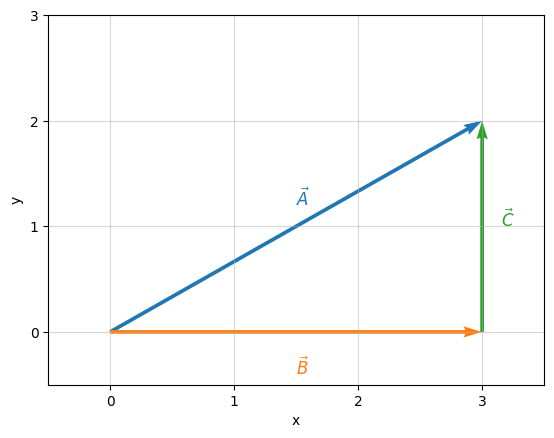
\includegraphics[width=0.55\linewidth]{Images/Kapittel1:introduksjon/Vektorer i xy_planet.png}
\end{center}
Deretter kan vi sette inn verdiene og finne ut hva $\vec{\mathrm{A}}$ er:
\begin{align*}
    \vec{\mathrm{B}} &= [3,0] = 3\hat{\mathbf{x}} + 0 \hat{\mathbf{y}}\\
    \vec{\mathrm{C}} &= [0,2] = 0 \hat{\mathbf{x}} + 2 \hat{\mathbf{y}}\\
    \vec{\mathrm{A}} &= (3+0)\hat{\mathbf{x}} + (0+2)\hat{\mathbf{y}} \\
    &= 3 \hat{\mathbf{x}} + 2 \hat{\mathbf{y}} = [3,2]
\end{align*}
Da får vi resultantvektoren $\vec{\textrm{A}} = [3,2]$.
}

\subsection*{Python: vektoraddisjon}

\begin{pythonkode}
import numpy as np

# Definer vektorene som NumPy-arrays
a = np.array([3.0, -1.0])
b = np.array([-1.0,  4.0])

c = a + b   # addisjon

print(f"a       = {a}")
print(f"b       = {b}")
print(f"a + b   = {c}")
print(f"|a + b| = {np.linalg.norm(c):.2f}")
\end{pythonkode}
\begin{pythonoutput}
a       = [ 3. -1.]
b       = [-1.  4.]
a + b   = [2. 3.]
|a + b| = 3.61
\end{pythonoutput}

\oppgave{Vektoraddisjon}{%
Gitt vektorene $\vec{a} = [3,\,-1]$ og $\vec{b} = [-1,\,4]$.
\begin{enumerate}[a)]
    \item Regn ut $\vec{a} + \vec{b}$.
    \item Regn ut $\vec{a} - \vec{b}$.
    \item Finn lengden til resultantvektoren $\vec{a} + \vec{b}$.
\end{enumerate}
}

\section{Skalarprodukt}

Skalarproduktet, også kalt prikkproduktet (engelsk: \textit{dot product}), er en operasjon mellom to vektorer som gir et tall (en skalar). Det uttrykker i hvilken grad to vektorer peker i samme retning.

\defn{Skalarprodukt}{Skalarproduktet av to vektorer $\vec{u} = [u_x,\, u_y]$ og $\vec{v} = [v_x,\, v_y]$ er definert som
\begin{align}
    \vec{u} \cdot \vec{v} = u_x\,v_x + u_y\,v_y.
\end{align}
Et ekvivalent uttrykk er
\begin{align}
    \vec{u} \cdot \vec{v} = |\vec{u}|\,|\vec{v}|\,\cos\theta,
\end{align}
der $\theta$ er vinkelen mellom vektorene.}

\paragraph{Geometrisk tolkning}

Skalarproduktet er et mål på \emph{hvor mye to vektorer peker i samme retning.} Tenk deg at vi slår lodd fra spissen av $\vec{A}$ ned på linjen til $\vec{B}$. Loddfoten gir en \emph{projeksjon} med lengde $|\vec{A}|\cos\theta$, og skalarproduktet er denne projeksjonen ganget med $|\vec{B}|$:
\[
\vec{A}\cdot\vec{B} \;=\;
\underbrace{|\vec{A}|\cos\theta}_{\text{projeksjon av }\vec{A}\text{ på }\vec{B}}
\;\cdot\; |\vec{B}|
\]

\begin{center}
\begin{tikzpicture}[scale=1.2]
  \draw[->, very thick, headCol] (0,0) -- (4.5,0) node[right] {$\vec{B}$};
  \draw[->, very thick, thmscol] (0,0) -- (2.5,1.75) node[above right] {$\vec{A}$};
  \node[above left=1pt, thmscol, font=\small] at (1.25,0.875) {$|\vec{A}|$};
  \draw[dashed, thmscol!55, thick] (2.5,1.75) -- (2.5,0);
  \draw (2.5,0) ++(-0.15,0) -- ++(0,0.15) -- ++(0.15,0);
  \draw[very thick, oppsumcol] (0,0) -- (2.5,0)
        node[midway, below=5pt] {$|\vec{A}|\cos\theta$};
  \draw[->, thick] (0.70,0) arc (0:35:0.70);
  \node[font=\small] at (0.98,0.22) {$\theta$};
\end{tikzpicture}
\end{center}

Spesielle tilfeller: $\theta=0^\circ$ (samme retning) $\Rightarrow$ $\cos\theta=1$ (maksimalt positivt); $\theta=90^\circ$ (vinkelrette) $\Rightarrow$ $\cos\theta=0$; $\theta=180^\circ$ (motsatt retning) $\Rightarrow$ $\cos\theta=-1$ (maksimalt negativt).

Ettersom vinkelen mellom enhetsvektorer i et ortogonalt system er 90°, gir definisjonen over oss følgende resultat:
\begin{align*}
\hat{\mathbf{x}} \cdot \hat{\mathbf{x}} = 1, \qquad
\hat{\mathbf{y}} \cdot \hat{\mathbf{y}} = 1, \qquad
\hat{\mathbf{x}} \cdot \hat{\mathbf{y}} = 0, \qquad
\hat{\mathbf{y}} \cdot \hat{\mathbf{x}} = 0.
\end{align*}
Her har vi brukt at enhetsvektorene har lengde 1, og at $\cos 90° = 0$ og $\cos 0° = 1$.

\exm{Skalarprodukt}{%
Finn skalarproduktet av $\vec{u} = 2\hat{\mathbf{x}} + 3\hat{\mathbf{y}}$ og $\vec{v} = 4\hat{\mathbf{x}} - \hat{\mathbf{y}}$.

\paragraph{Løsning:} Vi bruker definisjonen av skalarproduktet, og setter inn komponentene i forhold til enhetsvektorene:
\begin{align*}
\vec{u} \cdot \vec{v} &= (2\hat{\mathbf{x}} + 3\hat{\mathbf{y}}) \cdot (4\hat{\mathbf{x}} - \hat{\mathbf{y}}) \\
&= 2\cdot 4 (\hat{\mathbf{x}} \cdot \hat{\mathbf{x}}) + 2\cdot(-1) (\hat{\mathbf{x}} \cdot \hat{\mathbf{y}}) + 3\cdot 4 (\hat{\mathbf{y}} \cdot \hat{\mathbf{x}}) + 3\cdot(-1) (\hat{\mathbf{y}} \cdot \hat{\mathbf{y}}) \\
&= 8\cdot 1 + (-2)\cdot 0 + 12\cdot 0 + (-3)\cdot 1 \\
&= 8 - 3 = 5.
\end{align*}

}

\exm{Skalarprodukt og vinkel}{%
Finn skalarproduktet av $\vec{u} = [3,\,4]$ og $\vec{v} = [1,\,-2]$, og bestem vinkelen mellom dem.

\paragraph{Løsning:}
Komponentvis:
\[
\vec{u}\cdot\vec{v} = 3\cdot 1 + 4\cdot(-2) = 3 - 8 = -5.
\]
Størrelsen til vektorene er $|\vec{u}| = \sqrt{3^2+4^2} = 5$ og $|\vec{v}| = \sqrt{1^2+2^2} = \sqrt{5}$. Vinkelen finnes fra
\[
\cos\theta = \frac{\vec{u}\cdot\vec{v}}{|\vec{u}|\,|\vec{v}|} = \frac{-5}{5\sqrt{5}} = \frac{-1}{\sqrt{5}},
\]
altså $\theta = \arccos\!\left(-\dfrac{1}{\sqrt{5}}\right) \approx \doubleunderline{116.6^\circ}$.
}

\subsection*{Python: skalarprodukt og vinkel}

\begin{pythonkode}
import numpy as np

u = np.array([3.0,  4.0])
v = np.array([1.0, -2.0])

dot    = np.dot(u, v)
cos_th = dot / (np.linalg.norm(u) * np.linalg.norm(v))
theta  = np.degrees(np.arccos(cos_th))

print(f"u . v  = {dot}")
print(f"Vinkel = {theta:.1f} grader")
\end{pythonkode}
\begin{pythonoutput}
u . v  = -5.0
Vinkel = 116.6 grader
\end{pythonoutput}

\oppgave{Skalarprodukt}{%
Gitt $\vec{u} = [4,\,3]$ og $\vec{v} = [2,\,-1]$.
\begin{enumerate}[a)]
    \item Beregn skalarproduktet $\vec{u} \cdot \vec{v}$.
    \item Er vektorene vinkelrette? Begrunn svaret.
    \item Finn vinkelen mellom $\vec{u}$ og $\vec{v}$.
\end{enumerate}
}

\section{Kryssprodukt}

Kryssprodukt (engelsk: \textit{cross product}) er en operasjon mellom to vektorer som gir en ny vektor vinkelrett på begge. I to dimensjoner reduseres kryssproduktet til et enkelt tall — z-komponenten — som blant annet brukes til å beregne dreiemoment og areal av parallelogrammer.

\defn{Kryssprodukt i 2D}{For to vektorer $\vec{u} = [u_x,\, u_y]$ og $\vec{v} = [v_x,\, v_y]$ i $xy$-planet er kryssproduktets z-komponent
\begin{align}
    (\vec{u}\times\vec{v})_z = u_x\,v_y - u_y\,v_x.
\end{align}
Størrelsen til kryssproduktet er
\begin{align}
    |\vec{u}\times\vec{v}| = |\vec{u}|\,|\vec{v}|\,\sin\theta,
\end{align}
der $\theta$ er vinkelen mellom vektorene.}

Noen viktige egenskaper:
\begin{itemize}
    \item Dersom $\theta = 0^\circ$ (parallelle vektorer) er kryssproduktet \textbf{null}.
    \item Dersom $\theta = 90^\circ$ (vinkelrette vektorer) er størrelsen \textbf{maksimal}: $|\vec{u}\times\vec{v}|=|\vec{u}|\,|\vec{v}|$.
    \item Merk at kryssproduktet \emph{ikke} er kommutativt: $\vec{u}\times\vec{v} = -(\vec{v}\times\vec{u})$.
\end{itemize}

\exm{Kryssprodukt}{%
Finn kryssproduktet av $\vec{u} = [3,\,4]$ og $\vec{v} = [1,\,-2]$.

\paragraph{Løsning:}
\[
(\vec{u}\times\vec{v})_z = 3\cdot(-2) - 4\cdot 1 = -6 - 4 = \doubleunderline{-10}.
\]
Negativt fortegn betyr at den resulterende vektoren peker i negativ z-retning (inn i siden av arket).
}

\oppgave{Kryssprodukt}{%
Gitt $\vec{u} = [2,\,1]$ og $\vec{v} = [1,\,3]$.
\begin{enumerate}[a)]
    \item Finn $(\vec{u} \times \vec{v})_z$.
    \item Finn $(\vec{v} \times \vec{u})_z$.
    \item Hva kan du konkludere om kommutativitet for kryssproduktet?
\end{enumerate}
}

\section{Flere oppgaver}

Ingen oppgaver fra Øving~1 passer direkte til dette kapitlet. Oppgaver legges til etter hvert.
